\documentclass[border=6mm]{standalone}
\usepackage[utf8]{inputenc}
\usepackage[T1]{fontenc}
\usepackage{amsmath}
\usepackage{tikz}
\usetikzlibrary{arrows.meta, shadows.blur, shapes.geometric}
\definecolor{utnblue}{RGB}{0, 51, 102}

% Ej14a: ẏ + 3y = 2x  -->  y = (2/3)x - (1/3)ẏ
% Realización directa con derivadores, orden N=1.

\begin{document}
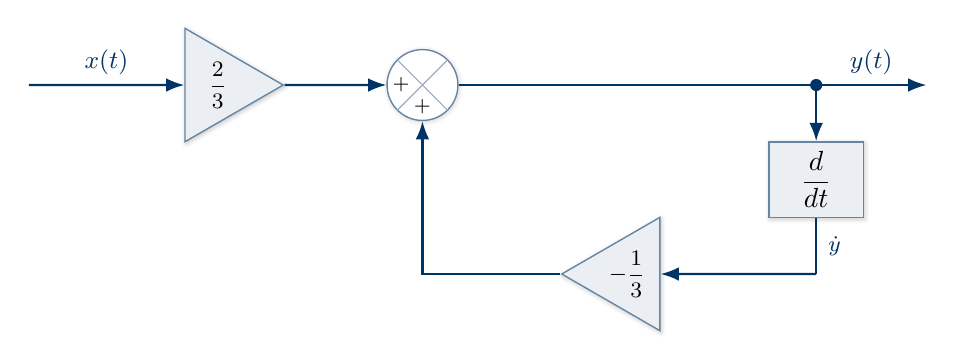
\begin{tikzpicture}[>=Latex, font=\small,
    gain_r/.style={
        regular polygon, regular polygon sides=3, shape border rotate=30,
        draw=utnblue!60, line width=0.5pt, fill=utnblue!8,
        minimum size=1.25cm, inner sep=0pt, font=\footnotesize,
        blur shadow={shadow blur steps=4, shadow blur extra rounding=0pt,
                     shadow xshift=0.4pt, shadow yshift=-0.6pt, shadow opacity=25}
    },
    gain_l/.style={
        regular polygon, regular polygon sides=3, shape border rotate=210,
        draw=utnblue!60, line width=0.5pt, fill=utnblue!8,
        minimum size=1.25cm, inner sep=0pt, font=\footnotesize,
        blur shadow={shadow blur steps=4, shadow blur extra rounding=0pt,
                     shadow xshift=0.4pt, shadow yshift=-0.6pt, shadow opacity=25}
    },
    op_block/.style={
        draw=utnblue!60, line width=0.5pt, fill=utnblue!8,
        minimum width=1.2cm, minimum height=0.9cm, font=\normalsize,
        blur shadow={shadow blur steps=4, shadow blur extra rounding=0pt,
                     shadow xshift=0.4pt, shadow yshift=-0.6pt, shadow opacity=25}
    },
    sum/.style={
        draw=utnblue!60, line width=0.5pt, circle,
        minimum size=0.9cm, inner sep=0pt, fill=white,
        blur shadow={shadow blur steps=4, shadow blur extra rounding=0pt,
                     shadow xshift=0.3pt, shadow yshift=-0.4pt, shadow opacity=20}
    },
    cross_line/.style={utnblue!40, line width=0.4pt},
    signal/.style={->, thick, utnblue},
    wire/.style={-, thick, utnblue},
    tlabel/.style={font=\footnotesize, inner sep=2pt},
]

% --- Coordenadas ---
\def\xinL{-5.0}
\def\xb{-2.6}
\def\xs{0}
\def\xa{2.6}
\def\xout{5.0}
\def\xoutR{6.4}

\def\yzero{0}
\def\ydone{-1.2}
\def\ytone{-2.4}

% --- Sumador con cruces internas ---
\node[sum] (S) at (\xs, \yzero) {};
\draw[cross_line] (-0.318, -0.318) -- (0.318,  0.318);
\draw[cross_line] (-0.318,  0.318) -- (0.318, -0.318);
\node[font=\scriptsize] at (-0.27,  0.00) {$+$};
\node[font=\scriptsize] at ( 0.00, -0.27) {$+$};

% --- Espina superior: x(t) -> [2/3] -> sum -> tap -> y(t) ---
\coordinate (in_left)   at (\xinL, \yzero);
\coordinate (out_tap)   at (\xout, \yzero);
\coordinate (out_right) at (\xoutR,\yzero);

\node[gain_r] (B0) at (\xb, \yzero) {$\dfrac{2}{3}$};

\draw[signal] (in_left) -- (B0.west) node[above, midway] {$x(t)$};
\draw[signal] (B0.east) -- (S.west);
\draw[wire]   (S.east) -- (out_tap);
\fill[utnblue] (out_tap) circle (2.2pt);
\draw[signal] (out_tap) -- (out_right) node[above, midway] {$y(t)$};

% --- Derivador en el lazo de la salida ---
\node[op_block] (Dout1) at (\xout, \ydone) {$\dfrac{d}{dt}$};
\coordinate (tout1) at (\xout, \ytone);

\draw[signal] (out_tap) -- (Dout1.north);
\draw[wire]   (Dout1.south) -- (tout1)
              node[tlabel, midway, anchor=west, xshift=2pt] {$\dot y$};

% --- Escalador de la salida (apunta a la izquierda) ---
\node[gain_l] (A1) at (\xa, \ytone) {$-\dfrac{1}{3}$};

\draw[signal] (tout1) -- (A1.east);

% --- Cable de realimentación ---
\draw[signal] (A1.west) -| (S.south);

\end{tikzpicture}
\end{document}
